\section{Systemtest med bruger-input}

\subsection{Beskrivelse}
For at teste det samlede system med bruger-input påsættes den positive og negative elektrode på femur, og referenceelektroden påsættes anklen, som illustreret i \autoref{sec:pilotforsoeg} på henholdsvis \autoref{fig:laarmuskler} og \autoref{fig:reference}, ud fra SENIAMs anvisninger \citep{seniam2016}. Huden præpareres inden dette for, således at fjerne hår og døde hudceller. 
De to accelerometre påsættes breadboards for at stabilisere deres placering, disse placeres henholdsvis parallelt med femur og tibia, som illustreret på \autoref{fig:accelerometervinkel}.

Systemet testes over 10 sekunders måling, hvor forsøgspersonen udfører en squat-øvelse. Der skal hertil foretages to målinger, hvor forsøgspersonen starter med at overskride 180$^{\circ}$ af knæet ved at overtrække knæleddet. Herefter bevæger forsøgspersonen sig langt ned i en squat-øvelse, hvorved vinklen af knæet overskrider grænsen på 90$^{\circ}$. Forsøgspersonen bevæger sig herefter tilbage til udgangsposition, hvorved de 180$^{\circ}$ overskrides ved overstræk af knæleddet.
På denne måde testes det, hvorvidt om det samlede system fungerer, da en overskridelse af $90-180^{\circ}$ vil betyde, at data ikke vil gå videre ind i EMG-algoritmen. Dette illustreres ved at det digitale output vil være i 0. Under testen opsamles det samplede digital filtrede EMG-signal, EMG-algoritmen samt vinklen over knæet.

\subsection{Resultater af forsøg}
På baggrund af testen er der plottet og visualiseret systemets input samt output. Visualiseringen forekommer af \autoref{fig:test_brugerinput}. 
 
\begin{figure}[H]
\centering
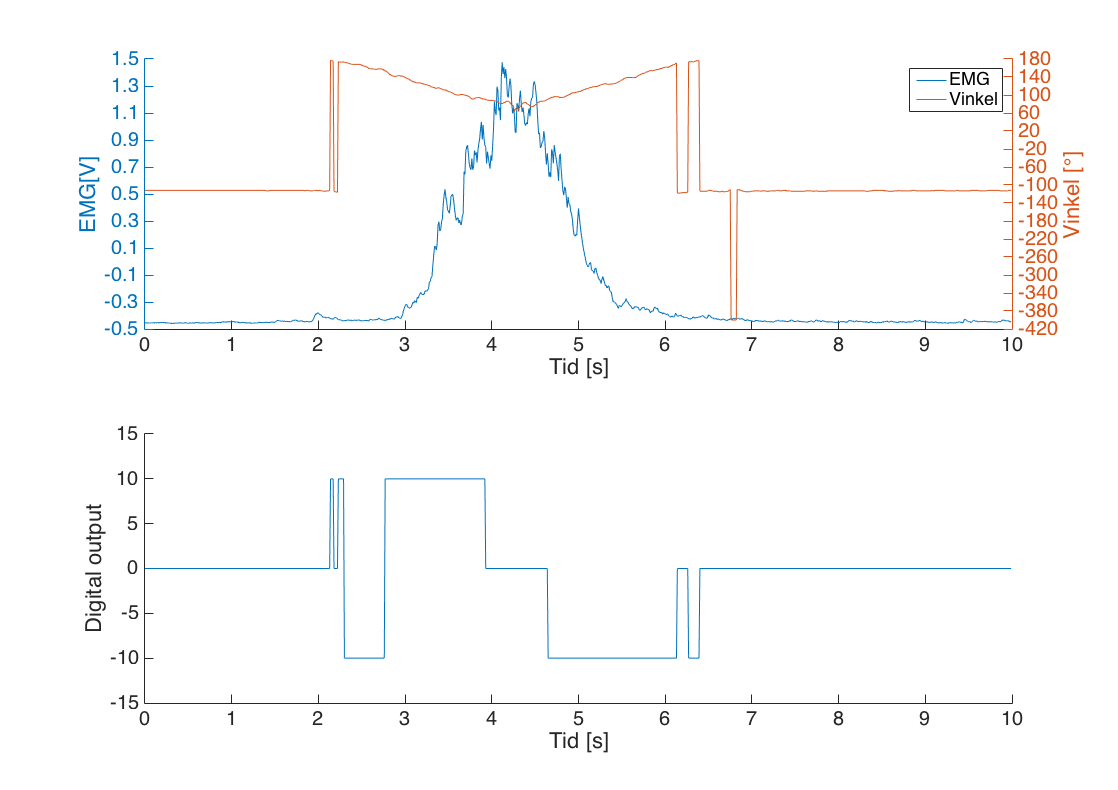
\includegraphics[width=0.4\textwidth]{figures/test_brugerinput}
\caption{På den øverste figur ses muskelaktivitet ved udførelse af en squat-øvelse, samt vinklen over knæet under øvelsen. Den blå graf illustrerer det samplede digital filtreret EMG og den røde graf illustrerer vinklen over knæet. Hertil ses der fald ned til under 0$^{\circ}$, hvilket illustrerer en overskridelse af $180^{\circ}$. Den nederste figur illusterer signalets digitale output i EMG-algoritmen. Denne visualiserer en stigning og et fald af det opsamlede EMG-signal, hvorved en stigning af muskelaktiviteten illustreres som værende $+10$ og et fald i muskelaktiviteten som værende $-10$. Ved grafen lig 0 illustreres en overskridelse af $90-180^{\circ}$ af knæet.}
\label{fig:test_brugerinput}
\end{figure}

Ud fra testen ses der en sammenhæng mellem muskelaktiviteten under en squat-øvelse og vinklen over knæet under øvelsen. Ved en stigning af muskelaktiviteten ses et fald i grader over knæet, hvilket ses mellem $2-4~s$. Hvorved der ved fald af muskelaktiviteten ses en stigning af grader, dette ses mellem $4,5-6,5~s$.
Ved starten af øvelsen overstrækker forsøgspersonen knæet, hvilket ses ved, at vinklen er $-112^{\circ}$. Grunden til denne er $-112^{\circ}$ og ikke $-400^{\circ}$ er, at det ene accelerometer har været indenfor græsen på $180^{\circ}$ og den andet accelerometer har overskredet grænsen. Det samme gør sig gældende ved slutningen af øvelsen. Ved overstrækning af knæet og dermed overskridelse af $180^{\circ}$ ses EMG-algorimten værende 0. 
Efter $2~s$ overstrækkes knæet ikke længere og graderne begynder derved at falde i takt med muskelaktiviteten stiger. Ved en stigning af muskelaktiviteten ses EMG-algorimten ligeledes stigende. Ved $4~s$ er vinklen over knæet $81^{\circ}$, hvilket er en overskridelse af grænsen på $90^{\circ}$. Dette illustreres ved EMG-algoritmen går i 0. 
Efter $4,5~s$ ses en stigning af grader i takt med et fald i muskelaktiviteten. Derved ses der ligeledes et fald i EMG-algoritmen. 
Efter $6~s$ overstrækkes knæene igen, hvorefter begge accelerometre overskrider deres grænser, derfor går grafen i $-400^{\circ}$. Herefter overstrækkes knæene fortsat, dog ligger det ene accelerometer indenfor dens grænse, hvilket forklarer vinklen på $-112^{\circ}$. 




\subsection{Konklusion}
